\documentclass[10pt,aspectratio=169]{beamer}

\usepackage{packages}
\usepackage{config}
\usepackage{appendixnumberbeamer}

\graphicspath{ {./images/} }

\title[Un motor de un solo qubit]{¿Eficiencia o entropía?}
\subtitle{Un motor de un solo qubit y la forma de sus mejores compromisos}
\author{Hugo Campos}
\institute[USM]{Universidad Técnica Federico Santa María\\[2pt]\small Termodinámica y Mecánica Estadística}
\date{Noviembre de 2026}
\titlegraphic{
\includegraphics[width=1.5cm]{Logo_UTFSM.png}}

\setbeamertemplate{navigation symbols}{}
\setlength{\parskip}{4pt}
\newcommand{\grande}[1]{{\Large #1}}
\newcommand{\nota}[1]{{\small\color{gray}#1}}
\newcommand{\clave}[1]{{\color{usmBlue}\bfseries #1}}

\begin{document}

%----------------------------------------------------------------- 1
\frame{\titlepage}

%----------------------------------------------------------------- 2
\begin{frame}{¿Qué le pedimos a un motor?}
\vspace{1.2em}
\begin{columns}[t]
\begin{column}{0.3\textwidth}\centering
  {\Huge\color{usmBlue}$P\,\uparrow$}\\[0.6em]
  \grande{Potencia}\\[0.3em]
  \nota{trabajo por unidad de tiempo}
\end{column}
\begin{column}{0.3\textwidth}\centering
  {\Huge\color{usmBlue}$\eta\,\uparrow$}\\[0.6em]
  \grande{Eficiencia}\\[0.3em]
  \nota{trabajo / calor absorbido}
\end{column}
\begin{column}{0.3\textwidth}\centering
  {\Huge\color{usmBlue}$\Delta P\,\downarrow$}\\[0.6em]
  \grande{Regularidad}\\[0.3em]
  \nota{fluctuaciones de la potencia}
\end{column}
\end{columns}
\vfill
\begin{center}
En un motor de \clave{un solo qubit} las tres compiten:\\ no se pueden tener a la vez.
\end{center}
\vspace{1em}
\end{frame}

%----------------------------------------------------------------- 3
\begin{frame}{Un qubit en contacto con un baño}
\begin{columns}[c]
\begin{column}{0.4\textwidth}\centering
  \begin{tikzpicture}[>=stealth]
    \draw[very thick, usmRed] (0,2) -- (2.6,2) node[right] {\small arriba: $\omega$};
    \draw[very thick, usmBlue] (0,0) -- (2.6,0) node[right] {\small abajo: $0$};
    \fill[usmYellow] (1.8,2) circle (5pt);
    \draw[<->, thick] (0.6,0.12) -- node[left] {\small brecha $\omega$} (0.6,1.88);
  \end{tikzpicture}

  \vspace{1.2em}
  Probabilidad de estar arriba (Gibbs):
  \[ a(\omega,T) = \frac{1}{1 + e^{\omega/T}} \]
  \nota{la brecha $\omega$ se controla desde afuera}
\end{column}
\begin{column}{0.56\textwidth}\centering
  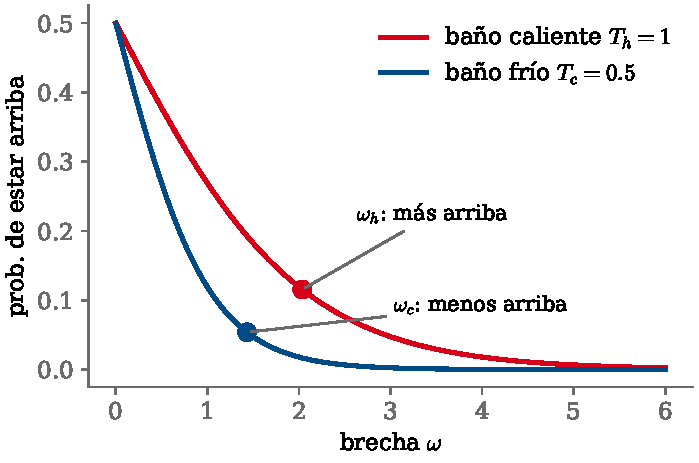
\includegraphics[width=\linewidth]{s_poblacion.pdf}
\end{column}
\end{columns}
\end{frame}

%----------------------------------------------------------------- 4
\begin{frame}{El ciclo de Otto: la brecha hace de volumen}
\begin{columns}[c]
\begin{column}{0.48\textwidth}\centering
  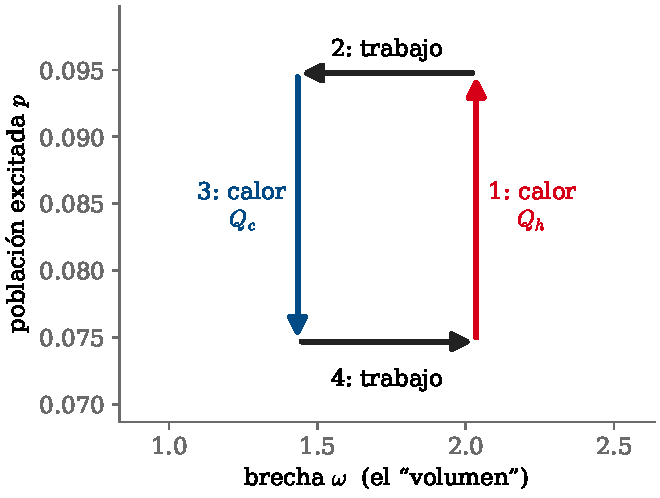
\includegraphics[width=\linewidth]{s_ciclo.pdf}
\end{column}
\begin{column}{0.48\textwidth}
  Primera ley, vista en mecánica estadística:
  \[
  \mathrm{d}E \;=\; \underbrace{\omega\,\mathrm{d}p}_{\text{calor}} \;+\; \underbrace{p\,\mathrm{d}\omega}_{\text{trabajo}}
  \]
  \nota{cambiar probabilidades es calor; cambiar niveles es trabajo}

  \vspace{1.5em}
  Eficiencia del ciclo:
  \[ \eta = 1 - \frac{\omega_c}{\omega_h} \;<\; \eta_C = 1 - \frac{T_c}{T_h} \]
\end{column}
\end{columns}
\end{frame}

%----------------------------------------------------------------- 5
\begin{frame}{Tiempo finito: el compromiso potencia--eficiencia}
\begin{center}
  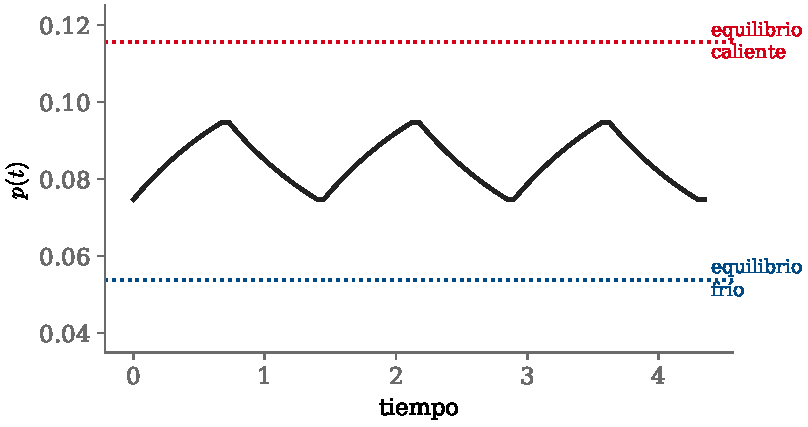
\includegraphics[width=0.62\linewidth]{s_pt.pdf}
\end{center}
\begin{columns}[t]
\begin{column}{0.45\textwidth}
  \clave{Contactos cortos:} no alcanza a pasar calor.\\
  \clave{Contactos largos:} la potencia se va a cero.
\end{column}
\begin{column}{0.45\textwidth}
  A potencia máxima: $\eta = 0{,}296$\\
  Curzon--Ahlborn: $1-\sqrt{T_c/T_h} = 0{,}293$
\end{column}
\end{columns}
\end{frame}

%----------------------------------------------------------------- 6
\begin{frame}{El trabajo fluctúa}
\begin{columns}[c]
\begin{column}{0.56\textwidth}\centering
  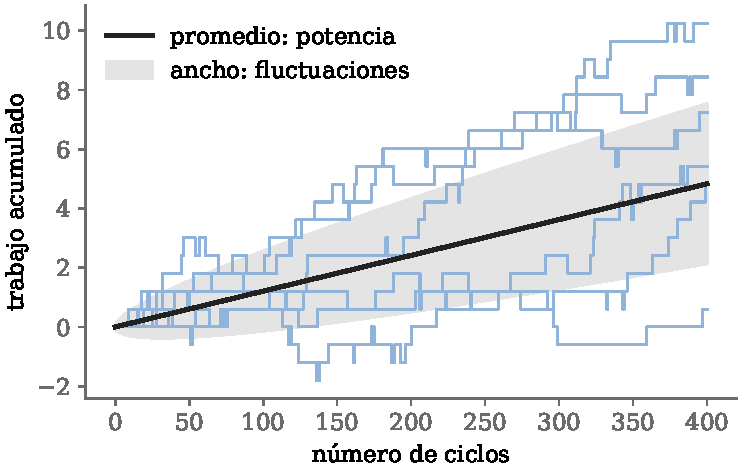
\includegraphics[width=\linewidth]{s_trayectorias.pdf}
\end{column}
\begin{column}{0.4\textwidth}
  Un qubit está \clave{arriba o abajo}, nunca ``al 9\%''.

  \vspace{0.6em}
  Trabajo de un ciclo:
  \[ w = \Delta\omega\,(s_1 - s_2) \]

  \vspace{0.3em}
  \nota{Media y varianza se calculan exactas con una función generadora que juega el papel de $\ln Z$.}
\end{column}
\end{columns}
\end{frame}

%----------------------------------------------------------------- 7
\begin{frame}{La relación de incertidumbre termodinámica}
\vspace{1.5em}
\begin{center}
  {\Huge $\Delta P \cdot \Sigma \;\ge\; 2P^2$}

  \vspace{0.8em}
  \nota{fluctuaciones $\times$ entropía producida $\ge$ 2 $\times$ potencia$^2$}

  \vspace{2em}
  \grande{La precisión \clave{cuesta disipación}.}

  \vspace{2em}
  Nuestros mejores motores están \clave{justo en el límite}:\\[0.3em]
  $\xi = \dfrac{2P^2}{\Delta P\,\Sigma} \approx 1$ \quad \nota{(mediana 0,996)}
\end{center}
\end{frame}

%----------------------------------------------------------------- 8
\begin{frame}{Optimizar tres cosas a la vez}
\begin{columns}[c]
\begin{column}{0.46\textwidth}\centering
  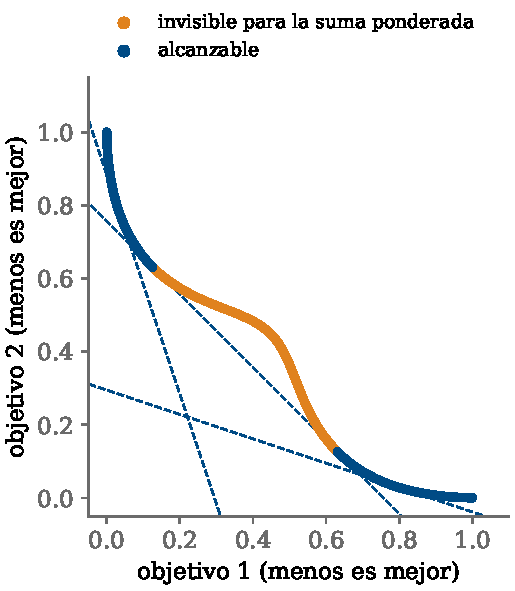
\includegraphics[width=0.85\linewidth]{s_envolvente.pdf}
\end{column}
\begin{column}{0.5\textwidth}
  No hay un mejor motor: hay un \clave{frente de Pareto}.

  \vspace{0.8em}
  La costumbre: una figura de mérito
  \[ F = a\,P + b\,\eta - c\,\Delta P \]
  y variar los pesos $a, b, c$.

  \vspace{0.8em}
  Problema: una suma ponderada es un plano que se desliza hasta tocar el frente.
  \clave{Solo ve la parte convexa.}
\end{column}
\end{columns}
\end{frame}

%----------------------------------------------------------------- 9
\begin{frame}{El resultado: silla contra tazón}
\begin{center}
  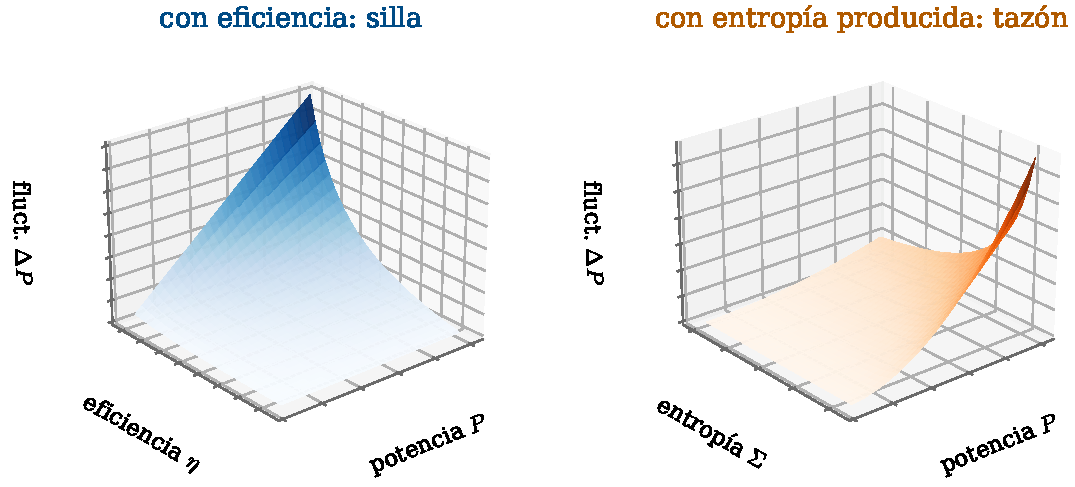
\includegraphics[height=0.5\textheight]{s_silla.pdf}
\end{center}
\vspace{-0.6em}
\begin{columns}[t]
\begin{column}{0.46\textwidth}\centering
  $\Delta P = \dfrac{2T_c\,\eta\,P}{\eta_C - \eta}$\\[0.3em]
  {\color{usmRed}ningún punto interior es alcanzable}
\end{column}
\begin{column}{0.46\textwidth}\centering
  $\Delta P = \dfrac{2P^2}{\Sigma}$\\[0.3em]
  {\color{usmGreen}todos los puntos son alcanzables}
\end{column}
\end{columns}
\vspace{0.8em}
\begin{center}
\clave{Los mismos motores}, otras coordenadas. \nota{$\eta$ es un cociente; $\Sigma$ es una cantidad que se suma.}
\end{center}
\end{frame}

%----------------------------------------------------------------- 10
\begin{frame}{Lo mismo que vimos en el curso}
\vspace{0.5em}
\begin{center}
\renewcommand{\arraystretch}{1.5}
\begin{tabular}{ll}
\toprule
\textbf{Mecánica estadística} & \textbf{Diseño del motor}\\
\midrule
entropía microcanónica $S(E)$ & frente de Pareto\\
temperatura $\beta$ & pesos $a, b, c$\\
energía libre: transformada de Legendre & figura de mérito óptima\\
construcción de Maxwell & lo que la suma ponderada no ve\\
\bottomrule
\end{tabular}
\end{center}
\vspace{1.2em}
\begin{center}
Si $S(E)$ no es cóncava, el ensamble canónico \clave{se salta} esos estados.\\
Si el frente no es convexo, la figura de mérito \clave{se salta} esos motores.
\end{center}
\end{frame}

%----------------------------------------------------------------- 11
\begin{frame}{¿Cuánto importa?}
\begin{center}
  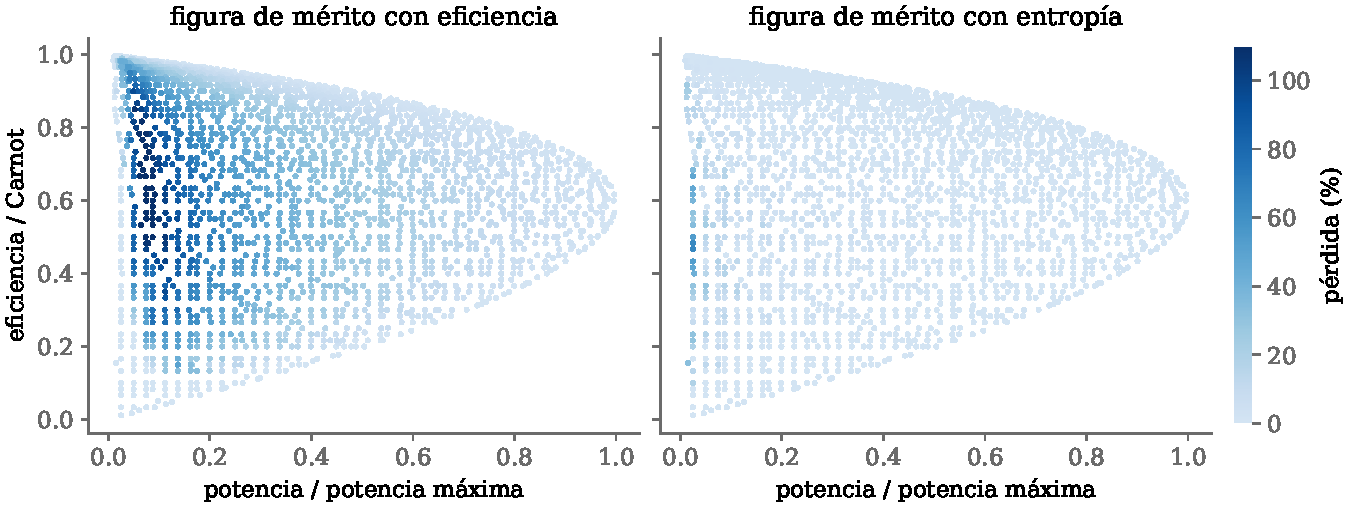
\includegraphics[width=0.9\linewidth]{s_costo.pdf}
\end{center}
\begin{columns}[t]
\begin{column}{0.44\textwidth}\centering
  Con $\eta$: alcanza el \clave{11\%} del frente;\\ pérdida mediana \clave{14\%}
\end{column}
\begin{column}{0.44\textwidth}\centering
  Con $\Sigma$: pérdida mediana \clave{0\%}
\end{column}
\end{columns}
\vspace{0.4em}
\begin{center}\nota{Se pierden los motores lentos, eficientes y de poco ruido.}\end{center}
\end{frame}

%----------------------------------------------------------------- 12
\begin{frame}{Conclusiones}
\vspace{1em}
\begin{enumerate}
\setlength{\itemsep}{1.4em}
\item[\color{usmBlue}\Large 1] \grande{La relación de incertidumbre \clave{fija la forma} de los mejores motores.}
\item[\color{usmBlue}\Large 2] \grande{Con $\eta$ esa forma es una \clave{silla}; con $\Sigma$, un \clave{tazón}.}\\
  \nota{Es la misma historia que Legendre y la construcción de Maxwell.}
\item[\color{usmBlue}\Large 3] \grande{Si usas una figura de mérito lineal, \clave{escríbela con $\Sigma$}.}
\end{enumerate}
\end{frame}

%----------------------------------------------------------------- cierre
{
\setbeamercolor{background canvas}{bg=usmBlue}
\setbeamertemplate{footline}{}
\begin{frame}[plain]
  \vfill
  \begin{center}
    {\color{white}\Huge ¡Gracias!}\\[10pt]
    {\color{white}\large ¿Preguntas?}
  \end{center}
  \vfill
\end{frame}
}

%================================================================= respaldo
\appendix

\begin{frame}{Respaldo 1: cómo se calculan las fluctuaciones}
Cada ciclo es una cadena de Markov. Se pesa cada salto por $e^{\chi w}$:
\[
\mathcal{T}(\chi)_{ss'} = \sum_{s_1} M^h_{s s_1}\, e^{\chi\Delta\omega s_1}\, M^c_{s_1 s'}\, e^{-\chi\Delta\omega s'},
\qquad
\theta(\chi) = \ln \lambda_{\max}\bigl(\mathcal{T}(\chi)\bigr)
\]
\vspace{0.3em}
\[
P = \frac{\theta'(0)}{\tau_{\text{ciclo}}}, \qquad \Delta P = \frac{\theta''(0)}{\tau_{\text{ciclo}}}
\]
\begin{itemize}
\item $\theta$ es el ``$\ln Z$'' del trabajo: derivarla da los cumulantes, con las correlaciones entre ciclos incluidas.
\item $\det\mathcal{T}$ no depende de $\chi$, así que todo sale en forma cerrada.
\item Validado con simulación Monte Carlo.
\end{itemize}
\end{frame}

\begin{frame}{Respaldo 2: siete algoritmos evolutivos (30 semillas)}
\begin{center}
  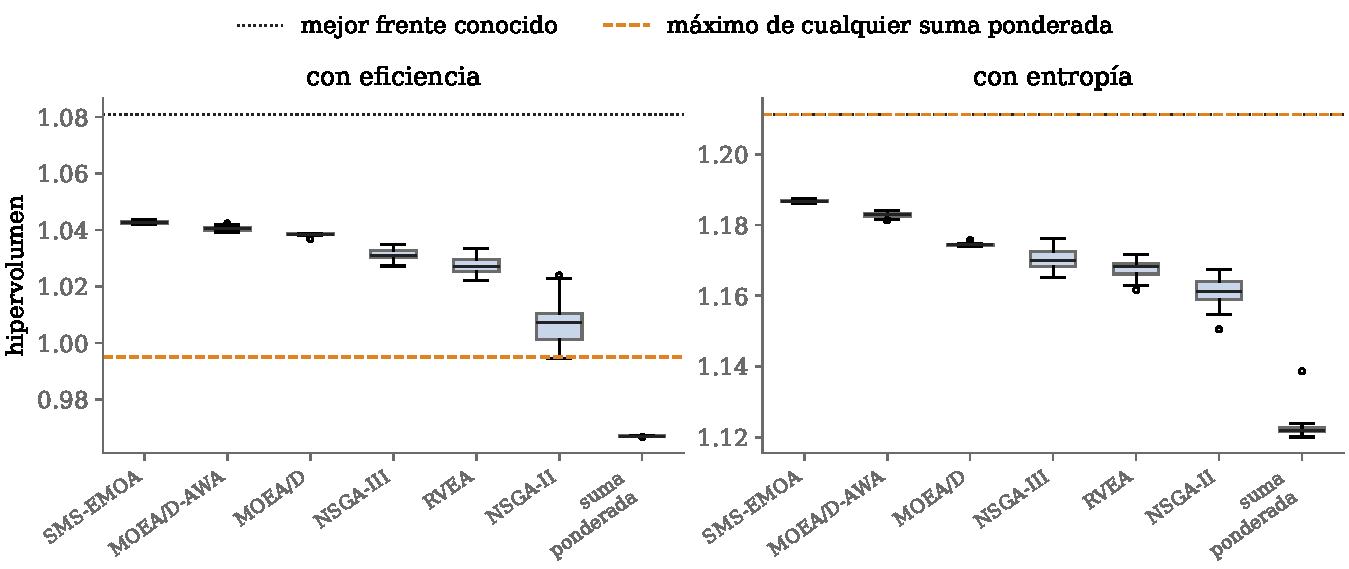
\includegraphics[width=0.92\linewidth]{s_hv_otto.pdf}
\end{center}
\begin{center}
Con $\eta$, \clave{6 de 7 algoritmos superan el máximo de cualquier suma ponderada}.\\
\nota{Con $\Sigma$ la suma ponderada pierde solo por amontonar soluciones, no por puntos inalcanzables.}
\end{center}
\end{frame}

\begin{frame}{Respaldo 3: cerca del equilibrio (respuesta lineal)}
\begin{columns}[c]
\begin{column}{0.52\textwidth}\centering
  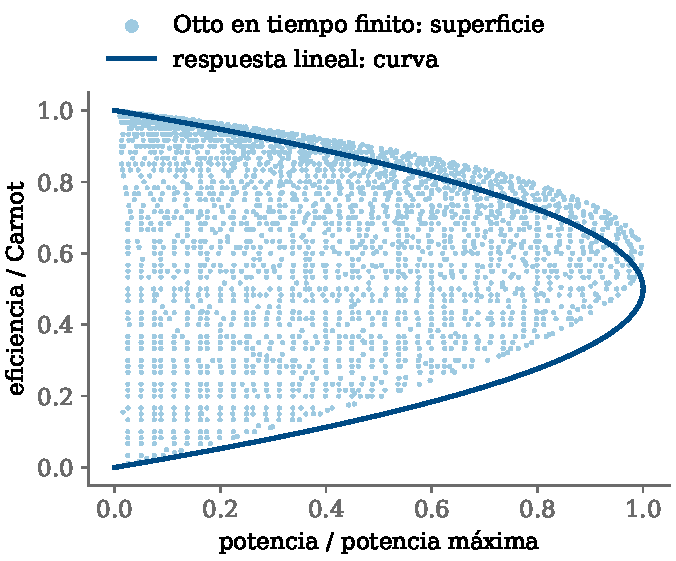
\includegraphics[width=\linewidth]{s_lr.pdf}
\end{column}
\begin{column}{0.44\textwidth}
  Con Onsager y acoplamiento fuerte, todo depende de \clave{un solo número} $e$:
  \[ P = e(1-e),\quad \bar\eta = e,\quad \Sigma = (1-e)^2 \]
  El frente es una \clave{curva}: la suma ponderada la encuentra entera.

  \vspace{0.5em}
  \nota{Almanza-Marrero, Roldán y Manzano (2026). Lejos del equilibrio, $P$ y $\eta$ se desacoplan y el frente pasa a ser una superficie.}
\end{column}
\end{columns}
\end{frame}

\begin{frame}{Respaldo 4: control libre por tramos}
\begin{center}
  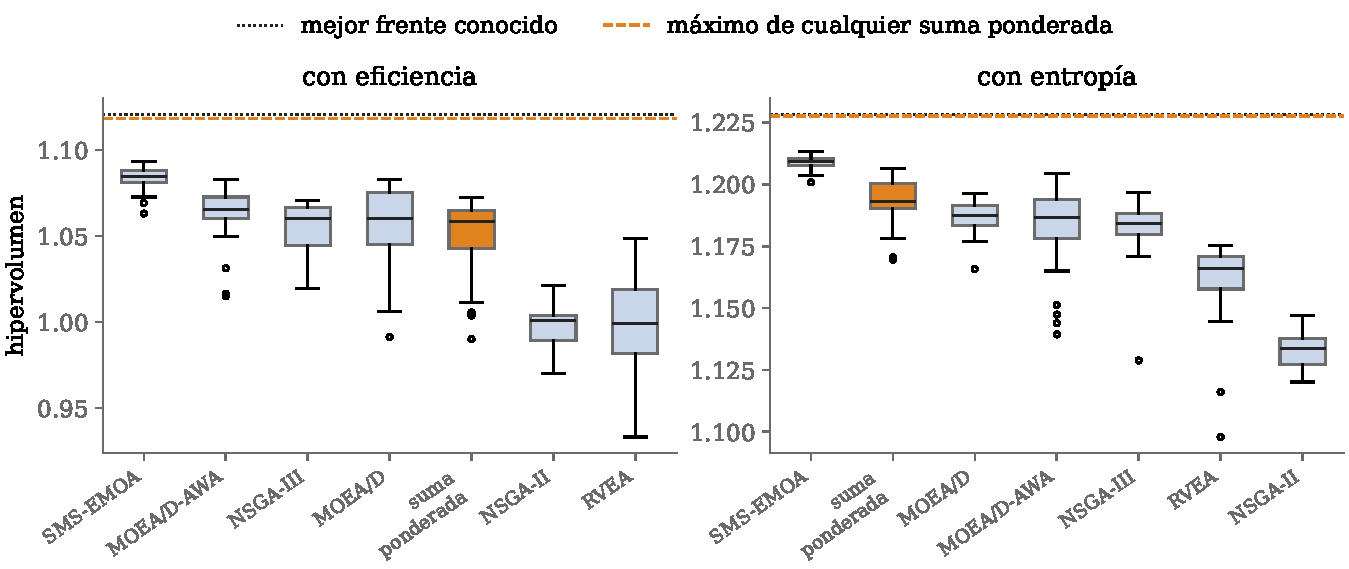
\includegraphics[width=0.88\linewidth]{s_hv_tramos.pdf}
\end{center}
\begin{center}
Con 8 tramos libres (modelo de Erdman et al.) la cota se rompe: $\xi$ hasta 4.\\
El frente queda \clave{casi convexo} en ambas coordenadas: el efecto está ligado a saturar la cota.
\end{center}
\end{frame}

\end{document}
